\chapter[Flujo en tuberías]{Flujo interno en tuberías}
\section{La ecuación de Darcy-Weisbach}
Cuando un fluido pasa por una tubería pierde energía debido a la fricción con las paredes. ésta pérdida de energía se mide normalmente como una pérdida de presión, ya que la velocidad está determinada por el caudal. Pero en realidad, se pierde una parte de la energía total, como se indica en la \textcolor{blue}{ecuación de Bernoulli generalizada}.

\begin{equation}
	p_1 + \frac{1}{2}\rho v_1^2 + \rho g z_1 = p_2 + \frac{1}{2}\rho v_2^2 + \rho g z_2 + \Delta p_f
\end{equation}


La pérdida de presión $\Delta p_f$ dependerá de la longitud $L$, el diámetro $D$ y la rugosidad $e$ de las paredes de la tubería y, por otra parte, de la velocidad media $v$, la densidad $\rho$ y la viscosidad $\mu$ del fluido,

\begin{equation}
	\Delta p_f = f(L,D,e,v,\rho,\mu).
\end{equation}

Son 7 variables. Del Teorema $\Pi$ de Buckingham sabemos que podemos reducirlas a 4 grupos adimensionales. La forma convencional de hacerlo es

\begin{equation}
	\frac{\Delta p_f}{\frac{1}{2} \rho v^2} = f\Bigl(\frac{L}{D},\frac{e}{D},\frac{\rho v D}{\mu}\Bigr)
\end{equation}


Es lógico pensar, y se comprueba experimentalmente, que ésta pérdida de presión ha de ser proporcional a la longitud $L$ de la tubería, de forma que

\begin{equation}
	\frac{\Delta p_f}{\frac{1}{2} \rho v^2} = \frac{L}{D} f\Bigl(\frac{e}{D},\frac{\rho v D}{\mu}\Bigr)
\end{equation}


$\frac{e}{D} = \varepsilon$ es la \textcolor{blue}{rugosidad relativa} de la tubería y $\frac{\rho v D}{\mu} = \re_D $ es el \textcolor{blue}{número de Reynolds} del flujo. y la expresión

\begin{equation}
	\boxed{
	\frac{\Delta p_f}{\frac{1}{2} \rho v^2} = \frac{L}{D} f(\varepsilon,\re_D)
}
\end{equation}

es la \textcolor{red}{ecuación de Darcy-Weisbach} (1850). $f$ es el \textcolor{red}{factor de fricción de Darcy}.


A veces es conveniente expresar la ecuación de Darcy-Weisbach en términos  de pérdida de altura, en lugar de pérdida de presión, $\Delta h_f = \frac{\Delta p}{\rho g}$,

\begin{equation}
	\Delta h_f = f(\varepsilon,\re_D) \frac{L}{D} \frac{1}{2g}v^2.
\end{equation}


\begin{center}
	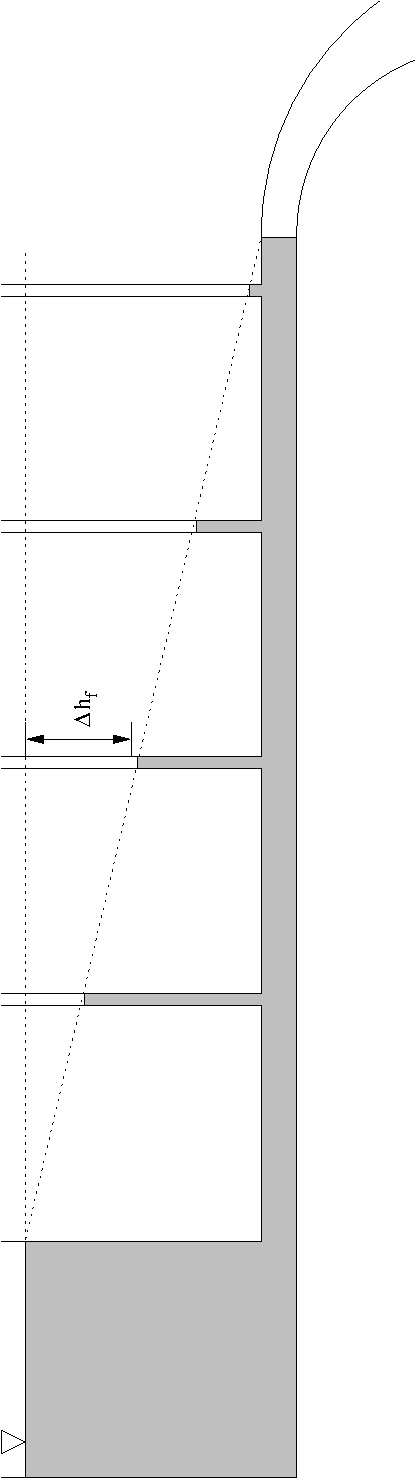
\includegraphics[scale=0.9,angle=270]{TeX_files/chapter10-Tuberias/alturas1.pdf}
\end{center}

\section{Flujo laminar}
Cuando $\re_D$ es pequeño (menor que aproximadamente 2300), en la tubería tenemos un flujo de Poiseuille, estudiado en el tema sobre Flujo Viscoso,

\begin{equation}
	v_x(r) = -\deriv{p}{x}\frac{1}{4\mu}\bigl(R^2 - r^2\bigr),
\end{equation}

donde ahora consideramos que el eje de la tubería está en la dirección $x$, y no hay variación de altura $z$.

$-\deriv{p}{x} = \frac{\Delta p_f}{L}$, y el hecho de que $\Delta p_f$ sea considerada una pérdida ya implica el signo negativo de la derivada,

\begin{equation}
	v_x(r) =  \frac{\Delta p_f}{L}\frac{1}{4\mu}\bigl(R^2 - r^2\bigr)
\end{equation}


La velocidad media del flujo es

\begin{equation}
	v = \frac{1}{S}\int_S v_x \dif S = \frac{1}{\pi R^2}\int_0^R v_x(r) 2\pi r \dif r = \frac{\Delta p_f}{L}\frac{R^2}{8\mu}.
\end{equation}

Vamos a ver cuánto vale $f$ en este caso,
\[\frac{1}{2g}v^2 = \frac{\Delta p_f}{L}\frac{R^2 v}{16\mu g} = \frac{\Delta p_f}{\rho g}\frac{D}{L}\frac{ \rho D v}{64\mu}\]
\[\frac{\Delta p_f}{\rho g} = h_f =\frac{64\mu}{ \rho D v}\frac{L}{D}\frac{1}{2g}v^2 \]

Por lo tanto,

\begin{equation}
	\boxed{
	f=\frac{64\mu}{ \rho D v} = \frac{64}{Re_D}
}
\end{equation}
que no depende de la rugosidad del material de la tubería.

\textbf{Ejemplo 1: }

Un aceite de densidad $\rho = 900 \,\text{Kg}/\text{m}^3$ y viscosidad $\nu = 2\times 10^{-4} \, \text{m}^2/\text{s}$ fluye hacia arriba por una tubería inclinada de 6 cm de diámetro, como se indica en la figura. Las presiones en los puntos 1 y 2, separados 10 metros, son $p_1 = 3.5\times10^5\,\text{Pa}$ y $p_2 = 2.5\times10^5\,\text{Pa}$, respectivamente. Vamos a calcular el caudal que circula por la tubería.

\begin{center}
	\input{TeX_files/chapter10-Tuberias/ejemplo1.eepicemu}
\end{center}

La ecuación de Bernoulli generalizada es
\[
p_1 + \frac{1}{2}\rho v_1^2 + \rho g z_1 = p_2 + \frac{1}{2} \rho v_2^2 + \rho g z_2 + \Delta p_f.
\]
Dado que no hay cambio de sección, $v_1 = v_2$, y la ecuación queda como
\[
p_1 + \rho g z_1 = p_2 + \rho g z_2 + \Delta p_f
\]
\[
\Rightarrow \, \Delta p_f = p_1 - p_2 + \rho g (z_1 - z_2) = \Delta p - \rho g L \sin \beta
\]

Supongamos que el flujo es laminar. En este caso,
\[
\Delta p_f  = f \frac{L}{D} \frac{1}{2} \rho v^2 = \frac{64}{\re_D} \frac{L}{D} \frac{1}{2} \rho v^2 = \frac{64 \nu}{v D} \frac{L}{D} \frac{1}{2} \rho v^2 =
\frac{32 \nu \rho L v}{D^2}.
\]
Igualando las dos expresiones,
\[
\frac{32 \nu \rho L v}{D^2} = \Delta p - \rho g L \sin \beta \, \Rightarrow \, v = \frac{D^2}{32 \nu \rho L} (\Delta p - \rho g L \sin \beta)
\]

Haciendo las operaciones obtenemos $v = 2.7 \, \text{m}/\text{s}$ y,
\[
Q = v \pi R^2 = 7.65\times10^{-3}\,\text{m}^3/\text{s}
\]

\section{Flujo turbulento en tubería lisa}
Supongamos que el perfil de velocidades sigue la ley logarítmica en toda la sección de la tubería\footnote{Ver capítulos sobre Turbulencia y Capa Límite.},

\begin{equation}
	\frac{v_x(r)}{v^*} \approx \frac{1}{\kappa}\ln \frac{(R-r)v^*}{\nu} + B,
\end{equation}

donde $(R-r)$ es la distancia hasta la pared.

\begin{center}
	\input{TeX_files/chapter10-Tuberias/turbulento1.eepicemu}
\end{center}


La velocidad media es
\[v = \frac{1}{S} \int_S v_x(r) \dif S = \frac{v^*}{\pi R^2}
\int_0^R \left[\frac{1}{\kappa}\ln \frac{(R-r)v^*}{\nu} + B\right] 2\pi r \dif r
\]

\begin{equation}
	v = \frac{v^*}{2} \left[\frac{2}{\kappa} \ln \frac{R v^*}{\nu} + 2B - \frac{3}{\kappa} \right]
\end{equation}

Si introducimos los valores conocidos $\kappa = 0.41$, $B=5.0$, obtenemos

\begin{equation}
	\frac{v}{v^*} = 2.44 \ln \frac{R v^*}{\nu} + 1.34
\end{equation}


La relación de esta velocidad media $v$ con la pérdida de presión en la tubería $\Delta p_f$ viene dada a través de $v^* = \sqrt{\frac{\tau_p}{\rho}}$.


Aplicando conservación de cantidad de movimiento sobre le Volumen de Control de la figura, considerando que el flujo es horizontal (no hay efectos de la gravedad) y estacionario, tenemos
\[
- p_1 S_1 + p_2 S_2 - \tau_p 2\pi R L = \dot{m}(v_2-v_1) = 0
\]
\[
\Rightarrow \, \Delta p_f \pi R^2 - \tau_p 2\pi R L = 0 \,
\Rightarrow \, \tau_p = \Delta p_f \frac{R}{2 L}
\]
de forma que la velocidad de fricción $v^*$ es

\begin{equation}
	v^* = \sqrt{\frac{\Delta p_f R}{2 \rho L}},
\end{equation}

y

\begin{equation}
	\frac{v}{v^*} = \frac{v}{\sqrt{\frac{\Delta p_f R}{2 \rho L}}} = \sqrt{\frac{2 \rho v^2 L}{R \Delta p_f}} = \sqrt{\frac{4 \rho v^2}{\Delta p_f}\frac{L}{D}} =
\sqrt{8\frac{1/2 \rho v^2}{\Delta p_f}\frac{L}{D}} = \sqrt{\frac{8}{f}}
\end{equation}


Por otro lado,
\[
\frac{R v^*}{\nu} = \frac{R}{\nu} \frac{v}{\sqrt{\frac{8}{f}}} = \frac{R v}{\nu}
\sqrt{\frac{f}{8}}= \frac{1}{2}\frac{D v}{\nu}\sqrt{\frac{f}{8}} = \frac{1}{2}\re_D\sqrt{\frac{f}{8}}
\]

De forma que podemos transformar la relación de la velocidad media $V$ en función de $v^*$ en una relación del factor de fricción $f$ en función de $\re_D$,

\begin{equation}
	\sqrt{\frac{8}{f}} = 2.44 \ln \left[\frac{1}{2}\re_D \sqrt{\frac{f}{8}}\right] + 1.34,
\end{equation}

que se suele expresar en términos de logaritmo en base 10, y con las constantes ajustadas para concordar con los experimentos, dando la \textcolor{red}{ecuación de Prandtl},

\begin{equation}
	\boxed{
	\frac{1}{\sqrt{f}} = 2.0\log \left[ \re_D \sqrt{f}\right] - 0.8
}
\end{equation}

Una relación explícita aproximada dada por Blasius es

\begin{equation}
	f = \frac{0.316}{\re_D^{1/4}}
\end{equation}

\begin{center}
	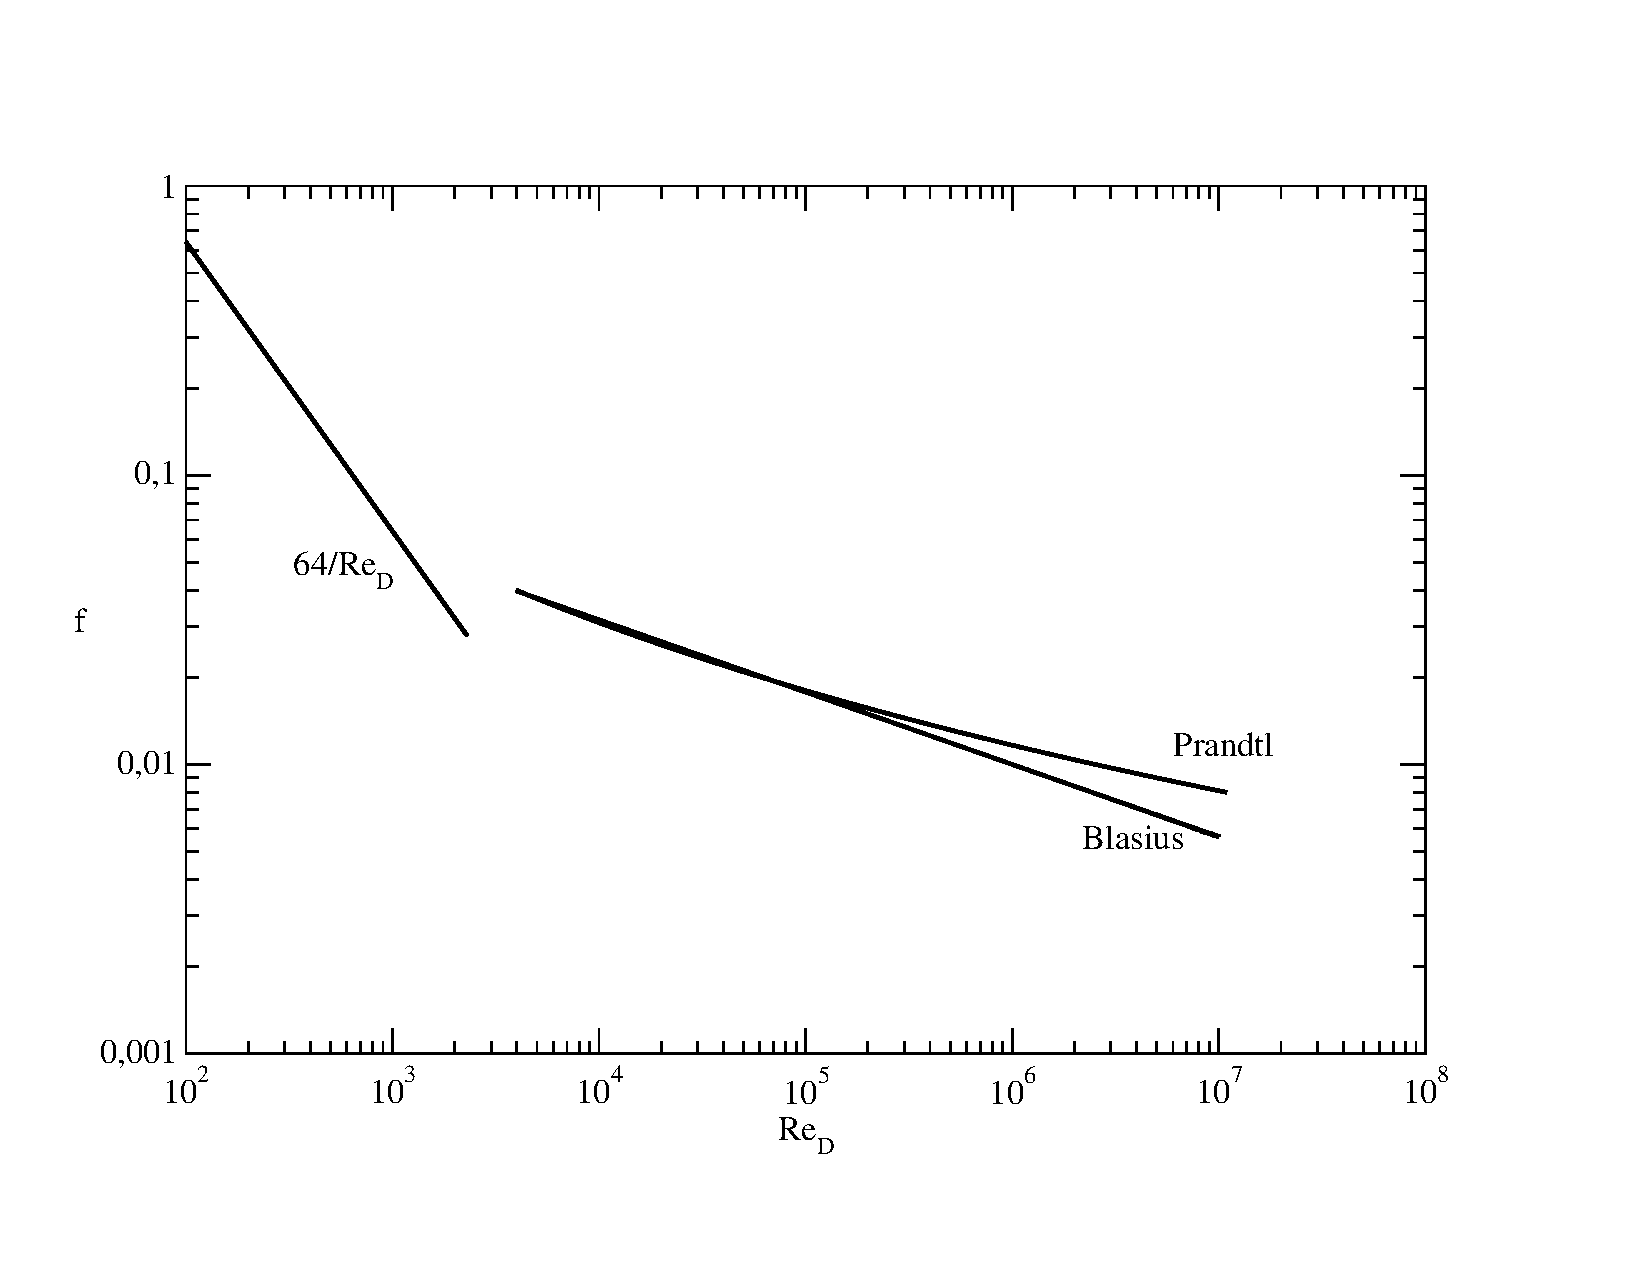
\includegraphics[scale=.45]{TeX_files/chapter10-Tuberias/f1.pdf}
\end{center}

\section{Flujo turbulento en tubería rugosa}

Nikuradse estudió el efecto que tiene la rugosidad de la tubería sobre el flujo turbulento, descubriendo que cuando la variable adimensional
$e^+ = \frac{e v^*}{\nu}$ es mayor que 70, el efecto sobre el flujo es indepediente de $\re_D$, y la velocidad en la ley logarítmica se reduce en una cantidad $\frac{1}{\kappa}\ln e^+ - 3.5$,
\[
\frac{v_x(r)}{v^*} = \frac{1}{\kappa}\ln \frac{(R-r) v^*}{\nu} + B - \bigl( \frac{1}{\kappa}\ln \frac{e v^*}{\nu}- 3.5\bigr) = \frac{1}{\kappa}\ln \frac{(R-r)}{e} + 8.5.
\]
Repitiendo el análisis anterior calculando  la velocidad media se llega a la relación entre $f$ y $\varepsilon$ con flujo completamente rugoso, en la que no hay dependencia con $\re_D$,
\[
\frac{v}{v^*} = -2.0\ln \frac{D}{e} + 3.2
\]

\begin{equation}
	\Rightarrow \,
\boxed{
	\frac{1}{\sqrt{f}} = -2.0 \log \frac{\varepsilon}{3.7}
}
\end{equation}

Más tarde Colebrook llegó a la expresión general que combinaba la relación para tubería lisa, y la del flujo completamente rugoso,

\begin{equation}
	\boxed{
	\frac{1}{\sqrt{f}} = -2.0 \log \left( \frac{\varepsilon}{3.7} + \frac{2.51}{\re_D \sqrt{f}} \right)
}
\end{equation}

y todas estas expresiones fueron condensadas en el \textcolor{red}{diagrama de Moody} que es la herramienta normalmente usada para el cálculo de pérdidas de presión en tuberías.

Indicación de algunas rugosidades típicas de materiales comunes usados en la construcción de tuberías

\begin{tabular}{|c|c|}
	\hline \textbf{Material}  & \textbf{rugosidad (mm)} \\
	\hline
	\hline Acero inox. nuevo & 0.002 \\
	\hline Acero comercial & 0.046 \\
	\hline Acero oxidado & 2.0 \\
	\hline Hierro de fundición & 0.26 \\
	\hline Hierro forjado & 0.046 \\
	\hline
\end{tabular}
\begin{tabular}{|c|c|}
	\hline \textbf{Material}  & \textbf{rugosidad (mm)} \\
	\hline
	\hline Hierro galvanizado & 0.15 \\
	\hline Fundición alfaltado & 0.12 \\
	\hline Hormigón  & 0.04 - 2.0 \\
	\hline Plástico & 0.0015 \\
	\hline Latón & 0.002 \\
	\hline
\end{tabular}
\newpage
\vspace*{-3cm}
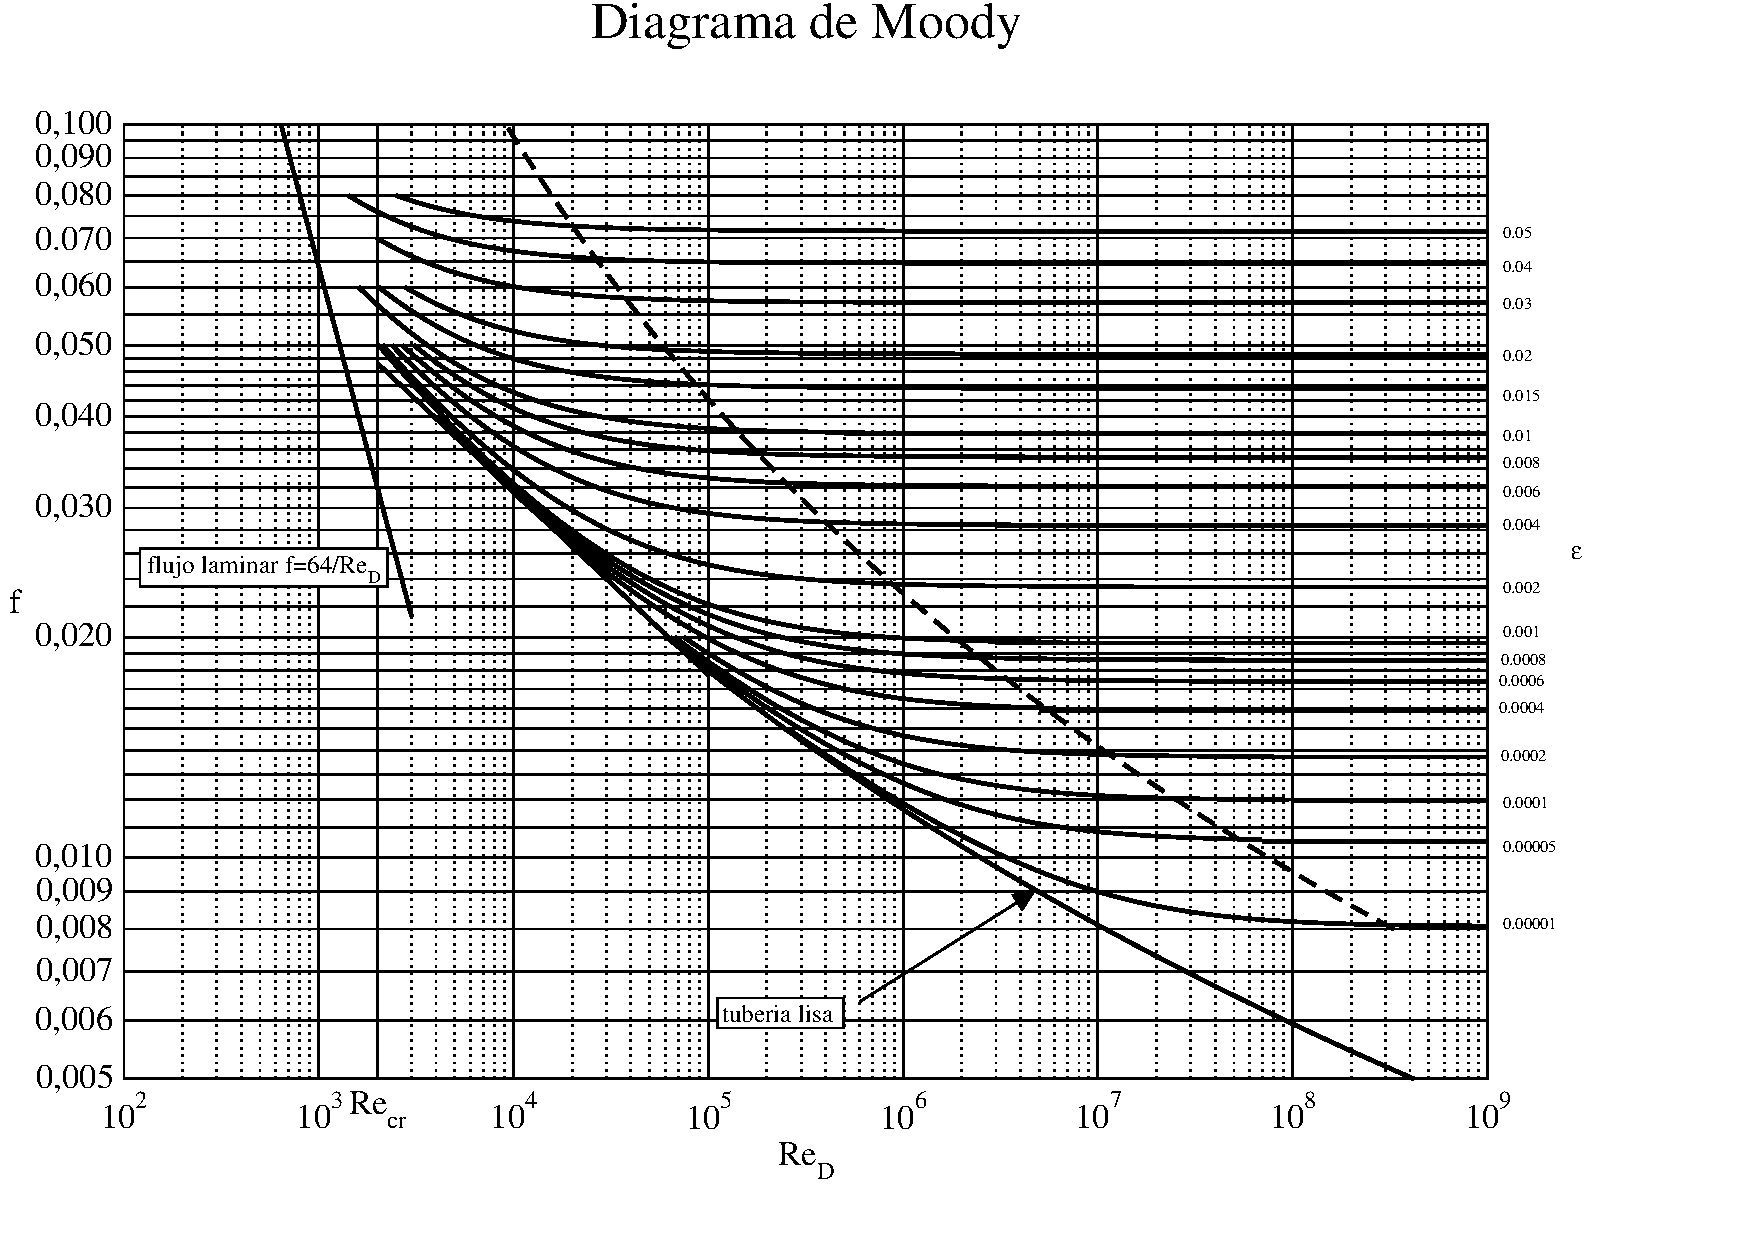
\includegraphics[scale=0.85,angle=90]{TeX_files/chapter10-Tuberias/moody.pdf}
\newpage
\textbf{Ejemplo :}

Queremos calcular la pérdida de presión en una tubería de fundición asfaltada de 150 mm de diámetro y 50 metros de longitud por la que circula agua con una velocidad media de 2,5 m/s.

En primer lugar calculamos $\re_D$ y la rugosidad relativa,
\[\re_D = \frac{v D}{\nu} = \frac{2.5\times 0.15}{10^{-6}} = 3.75\times10^5\]
\[\varepsilon = \frac{e}{D} = \frac{0.12}{150} = 8\times10^{-4}\]

Con estos valores estamos en la zona de flujo turbulento, aunque no es completamente rugoso, de forma que el factor de fricción va a venir dado por
\[
\frac{1}{\sqrt{f}} = -2.0 \log \left( \frac{\varepsilon}{3.7} + \frac{2.51}{\re_D \sqrt{f}} \right) = -2.0 \log \left( 2.162\times10^{-4} + \frac{6.693\times10^{-6}}{\sqrt{f}}\right)
\]

Hay, por lo menos, dos formas de resolver esta ecuación.

La primera es mediante un proceso iterativo. Iniciamos el cálculo con una aproximación de $f$ que podemos obtener del diagrama de Moody. Por ejemplo, $f_0=0.019$. Calculamos $f_1$ mediante
\[\frac{1}{\sqrt{f_1}} = -2.0 \log \left( 2.162\times10^{-4} + \frac{6.693\times10^{-6}}{\sqrt{f_0}}\right)\,\rightarrow\, f_1 = 0.01954
\]
y seguimos iterando
\[\frac{1}{\sqrt{f_2}} = -2.0 \log \left( 2.162\times10^{-4} + \frac{6.693\times10^{-6}}{\sqrt{f_1}}\right)\,\rightarrow\, f_2 = 0.01953
\]
hasta que obtenemos una convergencia suficiente.

La segunda es con una calculadora que resuelva ecuaciones de forma implicita (el proceso es el mismo, pero lo hace la calculadora de una forma mucho más rápida).

El valor correcto es $f= 0.01953$, de forma que la pérdida de presión es
\[\Delta p_f = f \frac{L}{D} \frac{1}{2}\rho v^2 = 0.01953 \times \frac{50}{0.15}\times\frac{1}{2}\times1000\times2.5^2 = 20340 \, \text{Pa}\]

\section{Cálculo de caudales}
Calcular la pérdida de presión $\Delta p_f$ a partir de los datos de la geometría de la tubería y las propiedades del fluido y su caudal es fácil.

Más interesante es calcular el caudal conocida la pérdida de presión. La forma de resolver este tipo de problemas es mediante un proceso iterativo, en el que se inicia considerando que el flujo es completamente rugoso, de forma que $f$ no dependa de $\re_D$
\[
\frac{1}{\sqrt{f_0}} = -2.0 \log \frac{\varepsilon}{3.7}
\]

Una vez tenemos $f$, calculamos la velocidad con
\[
\Delta p_f = f_0 \frac{L}{D} \frac{1}{2}\rho v_0^2
\]
y, de aquíel caudal.

Con esta velocidad se calcula ${\re_D}_0 = \frac{v_0 D}{\nu}$ y verificamos si el flujo es totalmente rugoso. Si es as\'{\i}, el problema está terminado. Si no, tenemos que volver a calcular $f_1$ mediante la expresión de Colebrook
\[
\frac{1}{\sqrt{f_1}} = -2.0 \log \left(\frac{\varepsilon}{3.7} + \frac{2.51}{\re_D \sqrt{f_1}}\right)
\]
e iterar hasta obtener la convergencia.

\textbf{Ejemplo : }

En una tubería de fundición asfaltada de 150 mm  de diámetro y 20 metros de largo, circula agua y la pérdida de presión es de 4 m.c.a. Queremos saber cuánto es el caudal de agua.

Suponemos flujo completamente rugoso con
\[\varepsilon = \frac{e}{D} = \frac{0.12}{150} = 8.0\times10^{-4}\]
y calculamos $f_0$,
\[
\frac{1}{\sqrt{f_0}} = -2.0 \log \frac{8.0\times10^{-4}}{3.7} \, \rightarrow \, f_0 = 0.0186
\]

El primer valor tentativo de la velocidad del flujo vendrá dado por
\[
\rho g h_f = f_0 \frac{L}{D}\frac{1}{2}\rho v_0^2
\]
\[
v_0 = \sqrt{\frac{g h_f 2 D}{f_0 L}} \, \rightarrow \, v_0 = 5.62 \, \text{m/s}.
\]

Calculamos el número de Reynolds
\[
{\re_D}_0 = \frac{v_0 D}{\nu}= 8.43\times 10^5
\]

Con este valor, no estamos en flujo completamente rugoso. De forma que volvemos a calcular el factor de fricción y la velocidad
\[
\frac{1}{\sqrt{f_1}} = -2.0 \log \left(\frac{8.0\times10^{-4}}{3.7}+\frac{2.51}{8.43\times 10^5\sqrt{f_1}}\right)
\]
\[
\rightarrow f_1 = 0.0190 \,\rightarrow \, v_1 = 5.56 \, \text{m/s}
\]

Si el grado de exactitud que se requiere no es muy elevado, podemos quedarnos con $v=5.6\,\text{m/s}$ y $Q=v\pi D^2/4 = 0.1 \, \text{m}^3/\text{s}$.

\section{Dimensionamiento de tuberías}

A veces se quiere saber cuál es el diámetro necesario de una tubería que debe llevar un determinado caudal con una pérdida de presión determinada. El problema no es sencillo, ya que para poder calcular $f$ es necesario $\re_D$ y $\varepsilon$, y los dos dependen del diámetro $D$.

Debemos de usar de nuevo un proceso iterativo. Iniciamos con un valor de $f$. Un valor típico és $f_0=0.02$.

A partir de este valor de $f$ calculamos el diámetro mediante
\[
\Delta p_f = f_0 \frac{L}{D}\frac{1}{2}\rho v_0^2 = \frac{8 f_0 \rho L Q^2}{\pi^2 D_0^5}
\]
\[
\Rightarrow  \, D_0 = \sqrt[5]{\frac{8 \rho f_0 L Q^2}{\pi^2 \Delta p_f}}
\]

Con este valor de $D_0$ calculamos $\varepsilon_0$ y ${\re_D}_0 = \frac{v_0 D_0}{\nu} = \frac{4 Q}{\pi D_0 \nu}$, y con estos valores  calculamos $f_1$, y continuamos el proceso iterativo hasta conseguir la convergencia deseada.

\textbf{Ejemplo : }

En el ejemplo anterior, queremos que el caudal sea el doble. ?` Cuál tendrá que ser el diámetro ?

Queremos que $Q=0.2\,\text{m}^3/\text{s}$. Iniciamos el proceso con $f_0=0.02$, y obtenemos
\[
D_0 = \sqrt[5]{\frac{8 \rho f_0 L Q^2}{\pi^2 \rho g h_f}} =
\sqrt[5]{\frac{8 f_0 L Q^2}{\pi^2 g h_f}} = 0.201\,\text{m}
\]

\[
\varepsilon_0 = \frac{e}{D_0} = \frac{0.12}{0.201} = 5.96\times10^{-4}
\]
\[
{\re_D}_0 = \frac{4 Q}{\pi D_0 \nu} = 1.27\times10^6
\]
\[
\frac{1}{\sqrt{f_1}} = -2.0 \log \left(\frac{5.96\times10^{-4}}{3.7}+\frac{2.51}{1.27\times 10^6\sqrt{f_1}}\right)
\, \rightarrow \, f_1 = 0.0177
\]
\[
D_1 = \sqrt[5]{\frac{8 f_1 L Q^2}{\pi^2 g h_f}} = 0.197\,\text{m}
\]
y seguiríamos quizás con una segunda iteración. Al final, de todas formas, hemos de escoger un medida de diámetro normalizada. En nuestro caso, 200 mm.

\section{Conductos no circulares}

Cuando el conducto no es circular los cálculos son más o menos los mismos, pero se complica un poco el álgebra.

Como medida equivalente al radio de la tubería se usa el concepto de \textcolor{red}{radio hidráulico}, definido como la relación entre la sección de paso del flujo y el perímetro mojado en el conducto

\begin{equation}
	R_h = \frac{A}{P}
\end{equation}


donde hay que tener en cuenta que $P$ es todo el perímetro en el que haya esfuerzo tangencial.

La pérdida de presión se calcula entonces como
\[
\Delta p_f = f \frac{L}{D_h} \frac{1}{2} \rho v^2
\]
donde $D_h = 4 R_h$ es el \textcolor{red}{diámetro hidráulico}, y $f$ es función de nuevo de la rugosidad relativa, $\varepsilon= e/D_h$ y el número de Reynolds se calcula como

\begin{equation}
	{\re_D}_h = \frac{v D_h}{\nu}.
\end{equation}


Por desgracia, para el cálculo de $f$ no sirven las expresiones deducidas para los conductos circulares ni el diagrama de Moody, aunque dan un valor bastante aproximado (dentro del 15\%) para flujo turbulento. Para flujo laminar el error es mayor, pero, por otro lado, el cálculo directo es más sencillo.

\textbf{Ejemplo : }

Calcular el factor de fricción $f$ para el flujo en un conducto rectabgular mucho mas ancho que alto ($b \gg h$) para flujo laminar y comparar con $f=64/\re_D$.

En este caso podemos considerar el flujo como el producido entre dos placas paralelas separadas por una distancia $h$. Sabemos que la distribución de velocidades es una parábola. Con el eje $z$ según la dirección del flujo y el eje $y$ perpendicular a las placas, tenemos
\[
v_z(y) = \frac{1}{\mu}\frac{\Delta p}{L}\left[y h -y^2\right]
\]

La velocidad media es
\[
v = \frac{1}{h}\int_0^h\frac{1}{\mu}\frac{\Delta p}{L}\left[y h -y^2\right] \dif y =
\frac{1}{12 \mu}\frac{\Delta p}{L} h^2
\]

Suponiendo que la velocidad es constante y que no hay ningún otro tipo de aporte o consumo de presión (gravedad, bombas, etc\ldots), la variación de presión $\Delta p$ és la pérdida de presión por fricción, $\Delta p_f$,
\[
\Delta p_f = \frac{12 \mu L v} {h^2}
\]

Vamos a relacionarlo con el número de Reynolds, que se define como
\[
\re_{D_h} = \frac{\rho D_h v}{\mu}
\]
donde $D_h = 4R_h = 4bh/(2a+2b)=2h$ si consideramos la aproximación $b \gg h$, de forma que, eliminado $\mu$ entre $\re_{D_h}$ y $\Delta p_f$, obtenemos
\[
\Delta p_f = \frac{24 \rho L v^2}{h\re_{D_h}} = \frac{96}{\re_{D_h}} \frac{L}{D_h} \frac{1}{2}\rho v^2
\]
es decir, $f ={96}/{\re_{D_h}}$, un 50\% más alto de lo correspondiente a un conducto circular.  La razón es que para un mismo diámetro hidráulico, un rectángulo siempre tiene mayor perímetro y, por lo tanto, mayor zona de actuación del esfuerzo tangencial de pared.


Para un conducto rectangular con $b \approx h$ el cálculo es mucho más complicado. Se suele usar entonces el concepto de \textcolor{red}{diámetro efectivo}, que es el diámetro que habría de tener un conducto circular que, en régimen laminar, tuviese la misma pérdida de carga con la misma velocidad media. Ya que para un conducto circular,

\begin{tabular}{lc}
	\begin{minipage}{0.5\textwidth}
		\[
		\Delta p_f = \frac{64}{\re}\frac{L}{D_e}\frac{1}{2}\rho v^2
		\]
		obtenemos
		\[
		\frac{64}{\re}\frac{L}{D_e}\frac{1}{2}\rho v^2 = f \frac{L}{D_h}\frac{1}{2}\rho v^2
		\]
		\[
		\Rightarrow \, D_e = \frac{64}{f \re} D_h
		\]
		donde $f\re$ se determina a partir de cálculos de la teoría laminar. éste diámetro se usa entonces también el cálculo de $f$ con flujo turbulento.
		
		\medskip 
		
	\end{minipage}
	&
	\begin{minipage}{0.4\textwidth}
		\begin{center}
			\begin{tabular}{|c|c|}
				\hline b/h & $f\re$ \\
				\hline
				\hline 0.0 & 96.00 \\
				\hline 0.05 & 89.91 \\
				\hline 0.1 & 84.68 \\
				\hline 0.125 & 82.34 \\
				\hline 0.167 & 78.81 \\
				\hline 0.25 & 72.93 \\
				\hline 0.4 & 65.47 \\
				\hline 0.5 & 62.19 \\
				\hline 0.75 & 57.89 \\
				\hline 1.0 & 56.91 \\
				\hline
			\end{tabular}
		\end{center}
	\end{minipage}
\end{tabular}

\bigskip

\textbf{Ejemplo : }

Por un conducto rectangular de $200\times 150$ mm y 30 metros de largo, con una rugosidad $e=0.1$~mm, circulan $0.7\, \text{m}^3/\text{s}$ de aire a $20^\circ C$ y 1 atmósfera de presión. Calcular la pérdida de presión.

La velocidad media del flujo es
\[
v = \frac{0.7}{0.03} = 23,3 \, \text{m/s}
\]
y el diámetro hidráulico es
\[
D_h = 4\frac{A}{P}=4\frac{ab}{2(a+b)}=\frac{2ab}{a+b}=171.43\,\text{mm}
\]

El diámetro efectivo es, de la tabla de $f\re$,
\[
D_e = \frac{64}{57.89}D_h = 189.5\,\text{mm}.
\]

Con este diámetro calculamos el factor de fricción,
\[
\re_{D_e}=\frac{v D_e}{\nu} = 2.5\times 10^5
\]
\[
\varepsilon = \frac{e}{D_e}=\frac{0.1}{189.5}=5.3\times10^{-4},
\]
usando el diágrama de Moody, $f=0.0185$, y la pérdida de presión
\[
\Delta p_f = f \frac{L}{D_e}\frac{1}{2}\rho v^2= 0.0185\times \frac{30}{0.1895}\times\frac{1}{2}1.2\times23.3^2 = 954\,\text{Pa}
\]

Si hubiésemos hecho el cálculo sin la corrección del diámetro efectivo, directamente con $D_e$, habríamos obtenido $\Delta p_f = 1087\,\text{Pa}$, es decir, un 15\% más grande. 

\section{Pérdidas de carga secundarias}

Además de la pérdida de carga provocada por fricción con las paredes de las tuberias y conductos, existen tamibén las {\it pérdidas de carga de forma, o secundarias}, creadas en puntos concretos de la instalación donde el flujo sufre cambios bruscos de módulo y/o dirección de la velocidad. Esto puede darse en:
\begin{itemize}
	\item Codos
	\item T's
	\item Bifurcaciones
	\item Válvulas
	\item Entradas/salidas de depósitos
	\item Filtros
	\item Toberas/difusores
	\item etc\ldots
\end{itemize}  

La pérdida de carga en estos elementos se caracteriza mediante el \textit{coeficiente de pérdidas secundarias}

\begin{equation}
	k = \frac{\Delta p_s}{\frac{1}{2}\rho v^2}
\end{equation}

donde $v$ es la velocidad del flujo en la tuber\'ia asociada al elemento.

Debido a la gran variedad de geometr\'ias y a la complejidad del flujo, no hay una teor\'ia que permita calcular el valor de $k$. éste viene dado por tablas o gráficas experimentales que a menudo, como en el caso de las válvulas, són facilitadas por el fabricante.

En general, se considera que el flujo es turbulento.


\begin{minipage}{10cm}
	Como ejemplo, mostramos el valor de $k$ para un codo de $45^\circ$, $90^\circ$ y $180^\circ$ en función de la relación entre el diámetro de la tuber\'ia $d$ y el radio de curvatura del codo$R$ 
	
	La forma de las gráficas es debida al efecto conjunto de la pérdida de carga primaria, que aumenta con $R/d$ y la secundaria, que disminuye.
	\medskip
	\begin{center}
		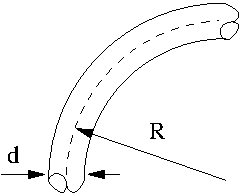
\includegraphics{TeX_files/chapter10-Tuberias/codo.pdf}
		% codo.eps: 300dpi, width=0.98cm, height=0.79cm, bb=0 0 116 93
	\end{center}
\end{minipage}
\begin{minipage}{10cm}
	\begin{center}
		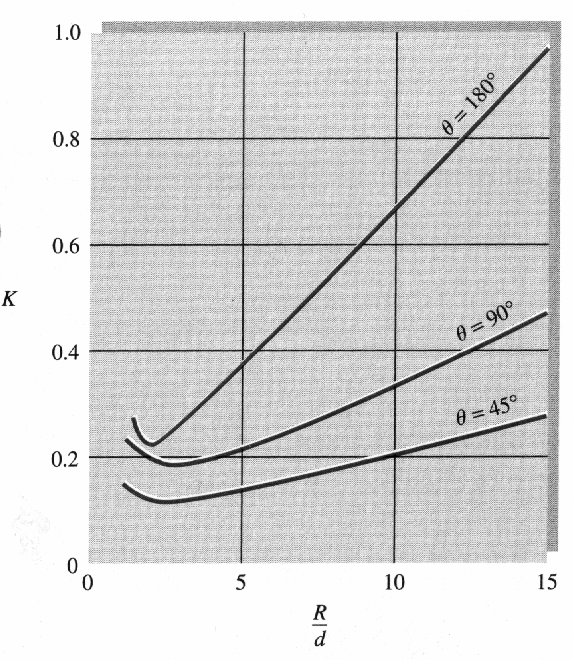
\includegraphics[width=5cm]{TeX_files/chapter10-Tuberias/k-codo.png}
		% k-codo.png: 200dpi, width=2.87cm, height=3.30cm, bb=0 0 226 260
	\end{center}
\end{minipage}

\begin{minipage}{10cm}
	En la salida brusca a un depósito, independientemente de la forma de ésta, $k=1$, debido a que, simplemente, se pierde la presión dinámica que lleva el flujo en la tuber\'ia. 
	
	Sin embargo, en la \textit{entrada de un depósito a una tuber\'ia}, el valor de $k$ depende fuertemente de la geometr\'ia, como se puede observar en las gráficas.
	\medskip
	\begin{center}
		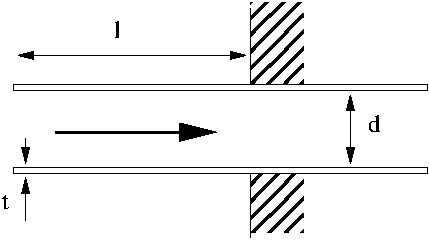
\includegraphics{TeX_files/chapter10-Tuberias/entrada_deposito.pdf}
	\end{center}
\end{minipage}
\begin{minipage}{10cm}
	\begin{center}
		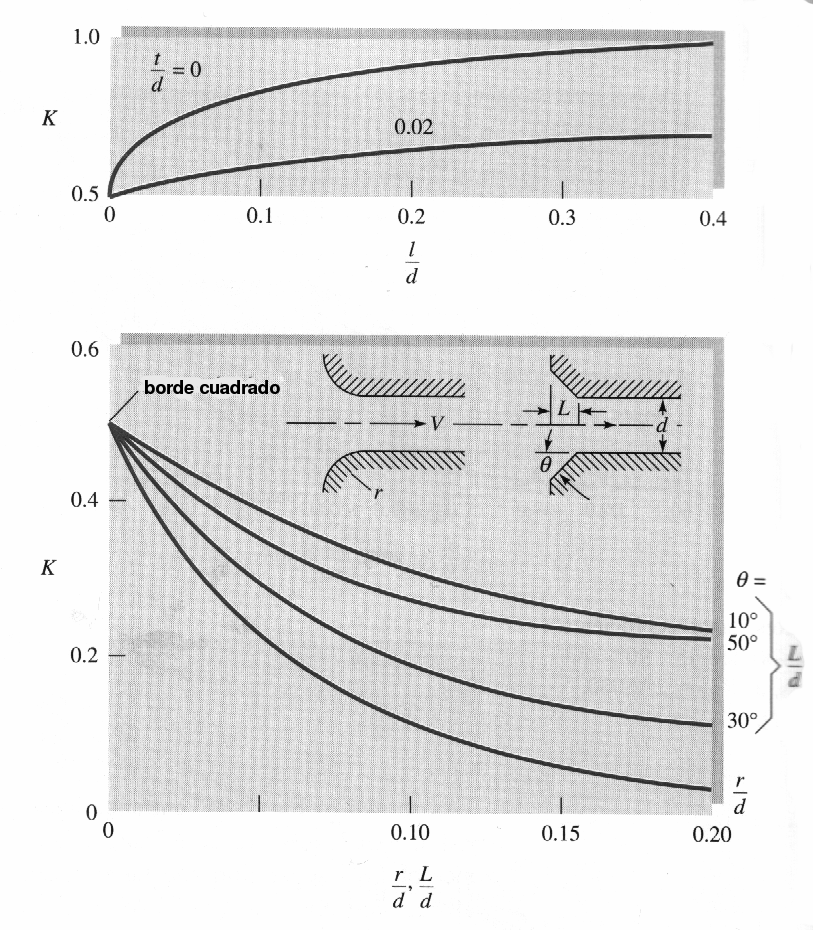
\includegraphics[scale=0.5]{TeX_files/chapter10-Tuberias/k-entrada-deposito.png}
	\end{center}
\end{minipage}

En una expansión, o contracción brusca, el valor de $k$ depende de la relación de diámetros de las tuber\'ias. En el caso de la expansión, el esfuerzo tangencial producido en la zona de aguas muertas es negligible, y un análisis simple de conservación de cantidad de movimiento y energ\'ia lleva a la expresión

\begin{minipage}{10cm}
	\[
	k = \left(1 - \frac{d^2}{D^2}\right)^2
	\]
	
	Para la contracción brusca, el flujo que llega de la tuber\'ia grande se contrae por debajo del diámetro de la tuber\'ia peque\~na, dando lugar a la vena contracta. Experimentalmente se encuentra que
	\[
	k \approx 0.42 \left(1 - \frac{d^2}{D^2}\right)
	\]
	si $d/D$ no es muy cercano a 1.
\end{minipage}
\begin{minipage}{10cm}
	\begin{center}
		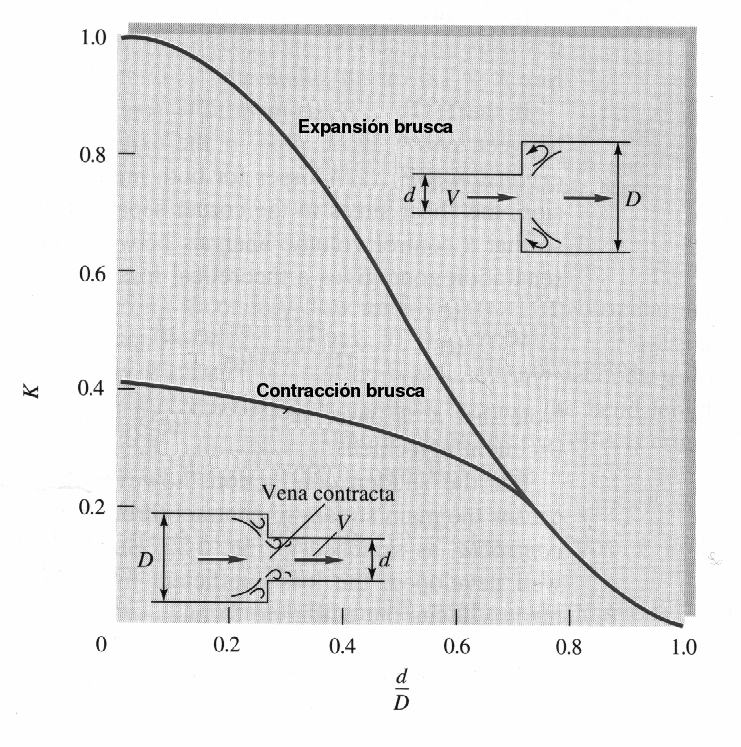
\includegraphics[scale=0.5]{TeX_files/chapter10-Tuberias/k-epansion-contraccion.png}
	\end{center}
\end{minipage}


Si la contracción es gradual, las pérdidas de carga secundarias son muy peque\~nas, y se pueden aproximar por los valores experimentales
\begin{center}
	% use packages: array
	\begin{tabular}{|c||c|c|c|}\hline
		$2\theta$ & 30 & 45 & 60 \\ \hline
		$k$ & 0.02 & 0.04 & 0.07 \\ \hline
	\end{tabular}
\end{center}

\begin{minipage}{10cm}
	Para una expansión gradual, también conocida como difusor, el valor de $k$ es como se muestra en la figura.
	
	El papel de un difusor es aumentar la presión estática del flujo. Esta caracter\'istica viene dada por el coeficiente de recuperación de presión
	\[C_p = \frac{p_2-p_1}{\frac{1}{2}\rho v_1^2}\]
\end{minipage}
\begin{minipage}{10cm}
	\begin{center}
		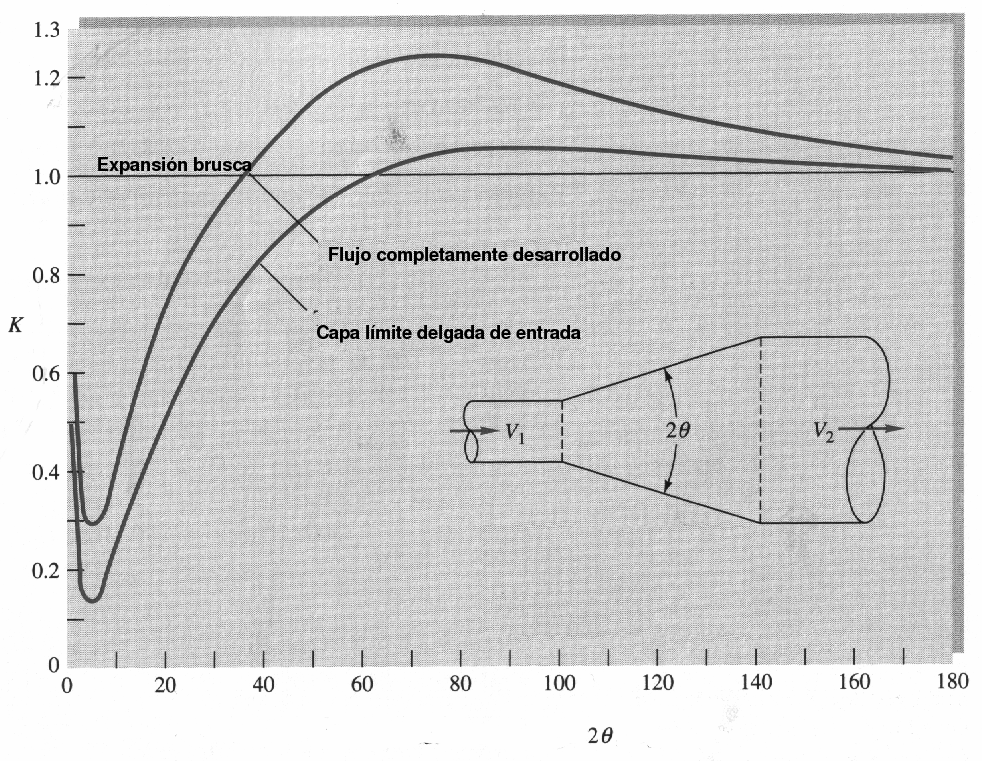
\includegraphics[width=5cm]{TeX_files/chapter10-Tuberias/difusor.png}
	\end{center}
\end{minipage}


El coeficiente de pérdida de carga secundaria y el coeficiente de recuperación de presión están relacionados mediante
\[k = 1- \frac{d_1^4}{d_2^4}-C_p\]

\textbf{Actividad:}

Demostrar esta expresión y discutir usando la gráfica, cuál es el mejor valor de $\theta$ para un difusor. ?`A qué es debido el aumento de $k$ para peque\~nos valores de $\theta$?
